%%%%%%%%%%%%%%%%%%%%%%%%%%%%%%%%%%%%%%%%%
% Beamer Presentation
% LaTeX Template

\documentclass{beamer}
\mode<presentation>{
% Theme
\usetheme{metropolis}
%\setbeamertemplate{footline} % To remove the footer line in all slides uncomment this line
%\setbeamertemplate{footline}[page number] % To replace the footer line in all slides with a simple slide count uncomment this line
%\setbeamertemplate{navigation symbols}{} % To remove the navigation symbols from the bottom of all slides uncomment this line
}

%Packages
\usepackage{graphicx} % Allows including images
\usepackage{booktabs} % Allows the use of \toprule, \midrule and \bottomrule in tables
%\usepackage{cite}
\usepackage[numbers]{natbib} % For bibliography
\usepackage{multirow}
\usepackage{hyperref}
%\usetheme{Warsaw}
\usepackage[absolute,overlay]{textpos}


% Prepare title and TOC
\title[Short title]{Reproducible Research} 
\author{Marco Chiapello} 
\institute[Center for Proteomics]{
Center for Proteomics\\
University of Cambridge \\ 
\medskip
\textit{mc983@cam.ac.uk} 
}
\date{27/03/2017} 

%\AtBeginSection[]
%{
%\begin{frame}<beamer>
%\frametitle{Overview}
%\tableofcontents[currentsection]
%\end{frame}
%}


%-------------------------------------------
% MAIN DOCUMENT
%-------------------------------------------
\begin{document}

%-------------------------------------------
% TITLE PAGE
%-------------------------------------------
\begin{frame}
\titlepage 
\end{frame}

%-------------------------------------------
% TABLE OF CONTENTS
%-------------------------------------------
\begin{frame}{Overview}
\small
\tableofcontents
\end{frame}

%----------------------------------------------------------------------------------------
%	PRESENTATION SLIDES
%----------------------------------------------------------------------------------------

\begin{frame}
\section{Introduction} 
\vspace{50px}
\begin{flushright}
\scriptsize {\bf Replication} is the ultimate standard by which scientific claims are judged \citep{Peng:2011et}\\
\scriptsize The fact that an analysis is {\bf reproducible does not guarantee the quality, correctness, or validity} of the published results. 
\end{flushright}
\end{frame}
%------------------------------------------------

\begin{frame}
\frametitle{What reproducible research is}
\begin{figure}
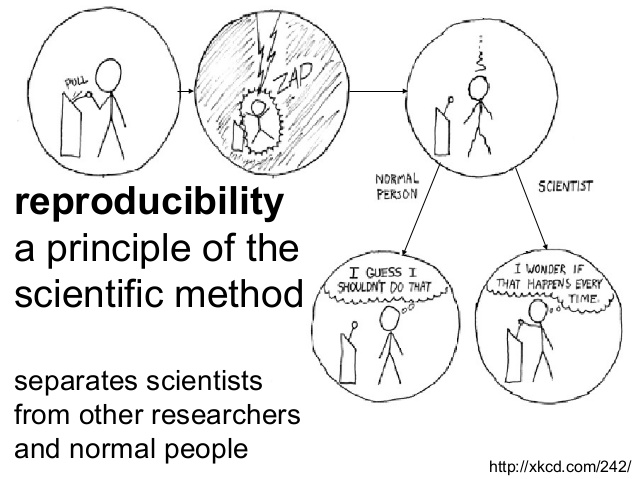
\includegraphics[scale=0.45]{figures/001.jpg}
\end{figure}
\end{frame}
%This slide contains a picture about reproducibility
%------------------------------------------------

\begin{frame}
\frametitle{What reproducible research is}
\begin{figure}
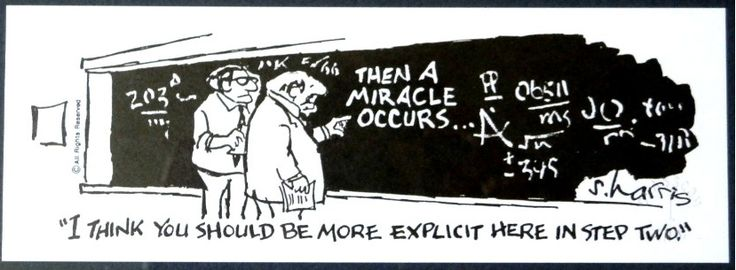
\includegraphics[scale=0.45]{figures/thenamiracleoccurs.jpg}
\end{figure}
\footnotesize
\begin{itemize}
	\item This is exactly how it seems when you try to figure out how authors got from a large and complex data set to a dense paper with lots of busy figures. \\Without access to the \textbf{data and the analysis code}, a miracle occurred.
\item And  there should be {\sc no miracles in science.} \citep{Markowetz:2016cs}
\end{itemize}
\end{frame}

%------------------------------------------------
\begin{frame}
\frametitle{What reproducible research is}
\Large\centering $DATA +  ANALYSIS \rightarrow RESULTS$\\
\rule{\textwidth}{0.05pt}\vspace{20px}
Common practice of writing statistical reports: 
\small\begin{itemize}
    \item We import a dataset into Excel
    \item Run a procedure to get the results
    \item Copy and paste selected pieces into a typesetting program (e.g. Word)
    \item Add a few descriptions
    \item Finish a report
\end{itemize}
\end{frame}


%------------------------------------------------
\begin{frame}
\frametitle{What reproducible research is}
\Large There are obvious dangers and disadvantages in this process:
\small\begin{enumerate}
	\item It is \textbf{error-prone} due to too much manual work;
	\item It requires lots of human effort to do \textbf{tedious jobs}; 
	\item The workflow is barely recordable, therefore it is \textbf{difficult to reproduce};
	\item A \textbf{tiny change} of the data source in the future will require the author(s) to go through the same procedure again;
	\item The analysis and writing are separate, so close attention has to be paid to the \textbf{synchronization of the two parts}.
\end{enumerate}
\end{frame}

%------------------------------------------------

\begin{frame}
\frametitle{What reproducible research is}
\Large \centering What is Reproducible Research?\\ 
{\sc The ability to reproduce someone else results}\\
\rule{\textwidth}{0.1pt}\\
\Large \centering What do you need?\\ 
\begin{itemize}
\item[--] Analytic data 
\item[--] Analytic code
\item[--] {\bf Documentation for data and code} 
\end{itemize}
\end{frame}


%------------------------------------------------

\begin{frame}
\frametitle{What reproducible research is}
\centering{\sc\Large Reproducible vs Replicable}
\begin{table}[]
\centering
\begin{tabular}{cccc}
                                           &                                & \multicolumn{2}{c}{DATA}                          \\ \cline{3-4}
                                           & \multicolumn{1}{c|}{}          & Same         & \multicolumn{1}{c|}{Different}     \\ \cline{2-4}
\multicolumn{1}{c|}{\multirow{2}{*}{CODE}} & \multicolumn{1}{c|}{Same}      & Reproducible & \multicolumn{1}{c|}{Replicable}    \\
\multicolumn{1}{c|}{}                      & \multicolumn{1}{c|}{Different} & Robust       & \multicolumn{1}{c|}{Generalisable} \\ \cline{2-4}
\end{tabular}
\end{table}
\vspace{3px}
\tiny Ref: {\url{https://github.com/KirstieJane/ReproducibleResearch}}
\end{frame}


%------------------------------------------------
\begin{frame}
\frametitle{What reproducible research is}

\Large{Reproducibility/reproduce}\\ \footnotesize A study is reproducible if there is a specific set of computational functions/analyses (usually specified in terms of code) that \textbf{exactly reproduce all of the numbers in a published paper from raw data}.

\Large{Replication/replicate}\\ \footnotesize A study is only replicable if you perform the exact same experiment (at least) twice, collect data in the same way both times, perform the same data analysis, and \textbf{arrive at the same conclusions}.
\rule{\textwidth}{0.05pt}
{\bf Reproducibility} is, to some extent, a technical challenge, while {\bf Replication} gives to the results scientific validity.
\rule{\textwidth}{0.05pt}\\
\vspace{3px}
\tiny Ref: {\url{https://github.com/lgatto/TeachingMaterial/tree/master/open-rr-bioinfo-best-practice}}
\end{frame}
%------------------------------------------------

\begin{frame}
\section{Reproducible research Reasons}
\vspace{50px}
\begin{flushright}
\scriptsize How does working reproducibly help to achieve more as a scientist \citep{Markowetz:2016cs}\\
\end{flushright}
\end{frame}
%------------------------------------------------

\begin{frame}
\frametitle{Reasons to work reproducibly}
\Large REPRODUCIBILITY \citep{Markowetz:2016cs}\\
Idealist:
\begin{enumerate}
\tiny
\item It is the foundation of science!
\item The world would be a better place if everyone worked transparently and reproducibly!
\end{enumerate}
\pause
Realist:
\begin{enumerate}
\footnotesize
\item It helps to avoid disaster
\begin{itemize}
\tiny
\item You need to record in detail how you got there
\item Work reproducibly early on will save you time later
\end{itemize}
\pause
\item It makes it easier to write papers
\begin{itemize}
\tiny
\item To have very transparent data and code, it costs just few minutes to spot a mistake (if any)
\end{itemize}
\pause
\item It helps reviewers see it your way
\begin{itemize}
\tiny
\item Made the data and well-documented code easily accessible to the reviewers
\end{itemize}
\pause
\item It enables continuity of your work
\begin{itemize}
\tiny
\item How can you ensure the continuity of work in your lab if progress is not documented reproducibly?
\item No proof of reproducibility, no result!
\end{itemize}
\pause
\item It helps to build your reputation
\begin{itemize}
\tiny
\item To build a reputation for being an honest and careful researcher
\end{itemize}
\end{enumerate}

\end{frame}

%------------------------------------------------
\begin{frame}
\section{Reproducible research Rules}
\vspace{30pt}
\scriptsize  
\raggedleft -- based on Sandve et al., 2013 \citep{Sandve:2013gh}
\end{frame}
%------------------------------------------------
\begin{frame}
\frametitle{Rule 1}
{\sc For Every Result, Keep Track of How It Was Produced}
\pause
\begin{itemize}
	\item The \textbf{full sequence} of pre- and post-processing steps are often critical in order to reach the achieved result
	\item \textbf{Every detail} that may influence the execution of the step \textbf{should be recorded}
    \item Include the name and version of the program, as well as the exact parameters and inputs
\end{itemize}
\begin{quote}As a minimum, you should at least record sufficient details on \underline{programs, parameters, and manual procedures} to allow yourself, in a year or so, to approximately reproduce the results\end{quote}
\end{frame}
%------------------------------------------------
\begin{frame}
\frametitle{Rule 2}
{\sc Avoid Manual Data Manipulation Steps}
\pause
\begin{itemize}
	\item Manual procedures are not only \underline{inefficient} and \underline{error-prone}, they are also difficult to reproduce
	\item Manual modification of files can usually be replaced by the use of standard \underline{UNIX commands} or scripts
	\item Manual tweaking of data files to attain format compatibility should be replaced by format converters that can be reenacted and included into executable workflows
	\item Manual operations like the use of \textbf{copy and paste} between documents should also be avoided
\end{itemize}
\begin{quote}
If manual operations cannot be avoided, you should as a minimum note down which data files were modified or moved, and for what purpose
\end{quote}

\end{frame}
%------------------------------------------------
\begin{frame}
\frametitle{Rule 3}
{\sc Archive the Exact Versions of All External Programs Used}
\pause
\begin{itemize}
	\item In order to exactly reproduce a given result, it may be necessary to use programs in the \textbf{exact versions used originally}
    \item It is not always trivial to get hold of a program in anything but the current version
\end{itemize}
\begin{quote}
    As a minimum, you should note the exact names and versions of the main programs you use
\end{quote}
\end{frame}
%------------------------------------------------
\begin{frame}
\frametitle{Rule 4}
{\sc Version Control All Custom Scripts}
\pause
\begin{itemize}
	\item \textbf{Only that exact state of the script may be able to produce that exact output}, even given the same input data and parameters
	\item The standard solution to \underline{track evolution of code} is to use a version control system
        \begin{itemize}[]
		\item \scriptsize A version control system is a repository of files with monitored access. \\ \textit{Every change made to the source is tracked, along with who made the change, why they made it}
        \end{itemize}
\end{itemize}
\begin{quote}
    As a minimum, you should archive copies of your scripts from time to time
\end{quote}
\end{frame}
%------------------------------------------------
\begin{frame}
\frametitle{Rule 5}
{\sc Record All Intermediate Results, When Possible in Standardized Formats}
\pause
\begin{itemize}
	\item In principle, as long as the \textbf{full process} used to produce a given result is tracked, all \textbf{intermediate data can also be regenerated}
	\item In practice, having easily \textbf{accessible intermediate results} may be of great value
    \item When the full process is not readily executable, it allows parts of the process to be rerun
    \item It \textbf{allows critical examination} of the full process behind a result
\end{itemize}
\begin{quote}
    As a minimum, archive any intermediate result files that are produced when running an analysis
\end{quote}
\end{frame}
%------------------------------------------------
\begin{frame}
\frametitle{Rule 6}
{\sc For Analyses That Include Randomness, Note Underlying Random Seeds}
\pause
\begin{itemize}
	\item Many analyses and predictions include some element of randomness, meaning the same program will typically give \textbf{slightly different results} every time it is executed
	\item Given the \textbf{same initial seed}, all random numbers used in an analysis will be equal, thus giving identical results every time it is run
\end{itemize}
\begin{quote}
    As a minimum, you should note which analysis steps involve randomness, so that a certain level of discrepancy can be anticipated when reproducing the results
\end{quote}
\end{frame}
%------------------------------------------------
\begin{frame}
\frametitle{Rule 7}
{\sc Always Store Raw Data}\
\pause
\begin{itemize}
	\item {\sc Always} store in a safe place the raw data
	\item {\sc Never} touch or mofidy the raw data
\end{itemize}
\end{frame}
%------------------------------------------------
\begin{frame}
\frametitle{Rule 8}
{\sc Generate Hierarchical Analysis Output, Allowing Layers of Increasing Detail to Be Inspected}
\pause
\begin{itemize}
	\item The final results that make it to an article, be it plots or tables, often represent \textbf{highly summarized data}
    \item In order to validate and fully understand the main result, it is often useful to inspect the detailed \textbf{values underlying the summaries}
    \item When working with summarized results, you should as a minimum at least once generate, inspect, and validate the detailed values underlying the summaries
\end{itemize}

\end{frame}
%------------------------------------------------
\begin{frame}
\frametitle{Rule 9}
{\sc Connect Textual Statements to Underlying Results}
\pause
\begin{itemize}
	\item The results of analyses and their corresponding textual interpretations are clearly interconnected but often \textbf{lie in different places}
    \item Results usually live on a personal computer, while interpretations live in text documents
    \item To allow efficient retrieval of details behind textual statements, we suggest that \textbf{statements are connected to underlying results} already from the time the statements are initially formulated
    \item {\bf Integrate reproducible analyses directly into textual documents}
\end{itemize}
\end{frame}
%------------------------------------------------
\begin{frame}
\frametitle{Rule 10}
{\sc Provide Public Access to Scripts, Runs, and Results}
\pause
\begin{itemize}
	\item All input data, scripts, versions, parameters, and inter-mediate \textbf{results should be made publicly and easily accessible}
	\item Making reproducibility of your work by peers a realistic possibility sends a \textbf{strong signal of quality, trustworthiness, and transparency}
\end{itemize}
\end{frame}
%------------------------------------------------
\begin{frame}
\section{Reproducible research Tools}
\begin{quote}
	\scriptsize    Let us change our traditional attitude to the construction of programs: Instead of imagining that our main task is to instruct a computer what to do, let us concentrate rather on \textbf{explaining to humans what we want the computer to do}.\\
\raggedleft   -- Donald E. Knuth Literate Programming, 1984
\end{quote}
\end{frame}
%------------------------------------------------
\begin{frame}
\frametitle{Tools}
\begin{center}\Large{\sc Folder organization}\end{center}
+-- README\\
+-- codeBook\\
+== rawdata\\
+== rscript\\
+== analysis\\
+== docs\\
+== manuscript\\
+== tmp
\end{frame}

%------------------------------------------------
\begin{frame}
\frametitle{Tools}
\begin{center}\Large{\sc A freely available language and environment for programming, computing and graphics}\end{center}

In this course we will use:
\begin{itemize}
	\item \texttt{UNIX}
	\item \texttt{R}
\end{itemize}
\end{frame}

%------------------------------------------------

\begin{frame}
\frametitle{Tools}
{\bf Literate programming} is a methodology that combines a programming language with a documentation language\\ 
\begin{itemize}
    \item Write program code to do computing
    \item Write narratives to explain what is being done by the program code
\end{itemize}
\end{frame}

%------------------------------------------------

\begin{frame}
\frametitle{Tools}
\begin{center}\Large\texttt{R}Markdown\end{center}
\begin{center}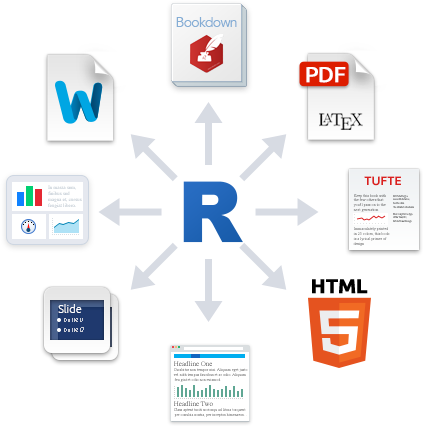
\includegraphics[scale=0.35]{figures/RMarkdownOutputFormats.png}\end{center}
\begin{center}\tiny Ref: {\url{http://rmarkdown.rstudio.com/index.html}}\end{center}
\end{frame}
%-----------------------------------------------
\begin{frame}
\frametitle{Tools}
\begin{center}\Large\texttt{R}Markdown\end{center}
\begin{center}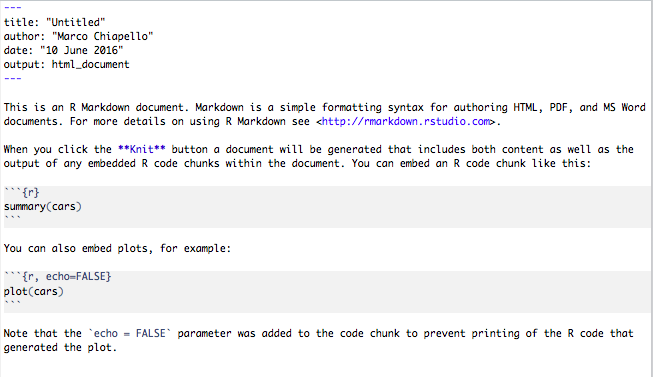
\includegraphics[scale=0.45]{figures/RMarkdown.png}\end{center}
\end{frame}
%------------------------------------------------
\begin{frame}
    \frametitle{Tools}
    \begin{center}\Large {\sc Version Control}\end{center}
\begin{center}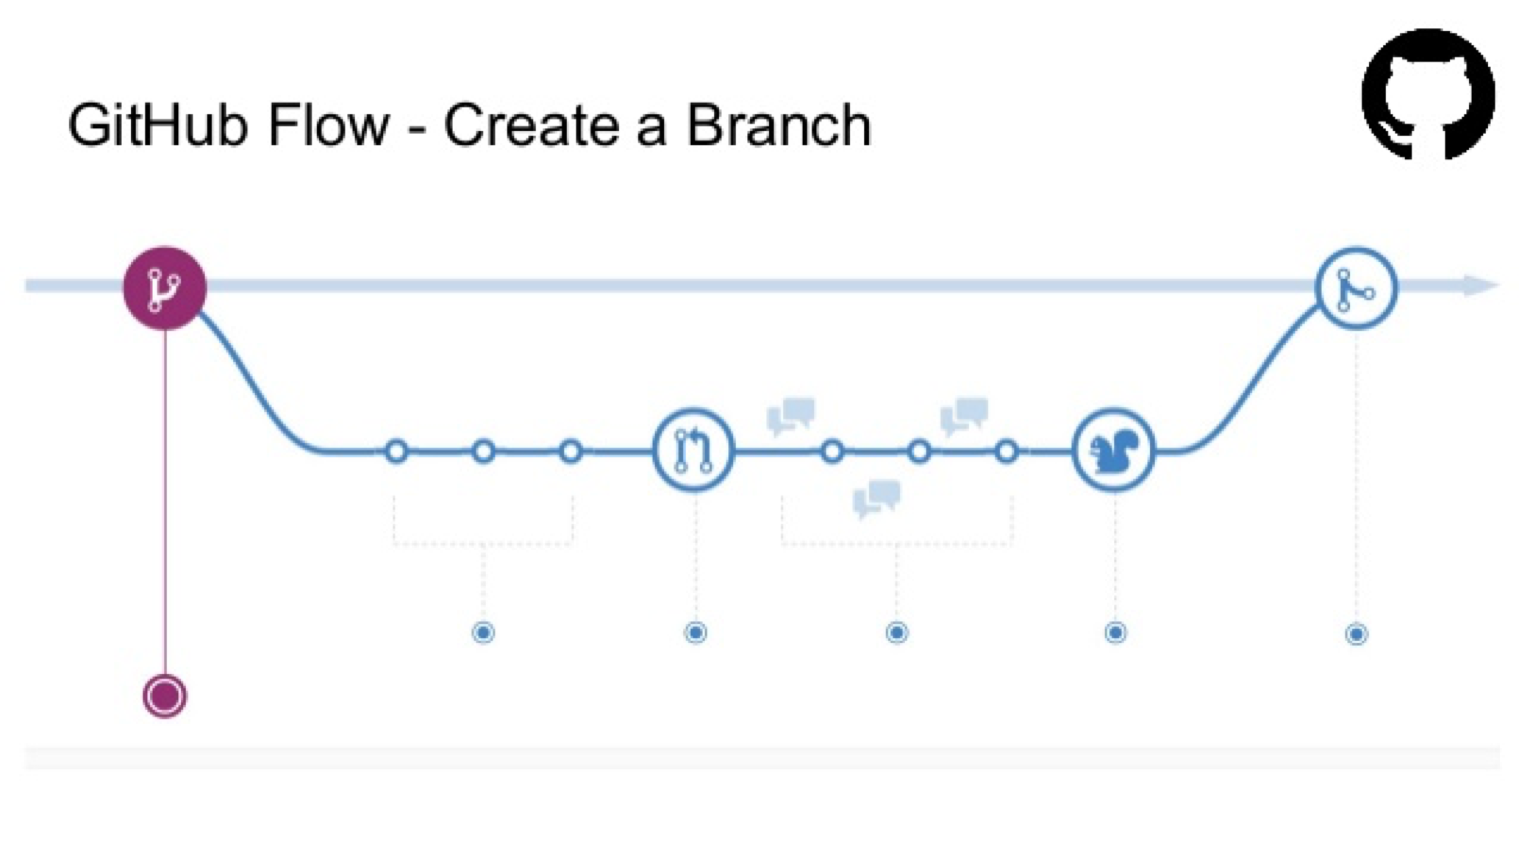
\includegraphics[scale=0.45]{figures/git.png}\end{center}

\end{frame}
%------------------------------------------------
\begin{frame}
\frametitle{Tools}

Learning to use these tools will require \textbf{commitment} and a \textbf{massive investment of your time and energy}.\\ 
A priori it is not clear why the benefits of working reproducibly outweigh its costs.\\

{\bf Does reproducibility sound like extra work?}\\
It can be, particularly when one is first trying to do it, that is, to break one's own previous nonreproducible habits


\end{frame}

%------------------------------------------------
\section{Conclusion}
%------------------------------------------------

\begin{frame}
\frametitle{Conclusions}

\begin{center}\Huge{\sc My advice is:}\\ \vspace{20pt}
    \Large Learn the tools of reproducibility as quickly as possible and use them in every project.\end{center}
\end{frame}

%------------------------------------------------

\begin{frame}
\frametitle{References}
\fontsize{6}{7.2}\selectfont
\bibliographystyle{apalike}
\bibliography{bib2}
\end{frame}
%------------------------------------------------

\end{document}
